%%\documentclass[a4paper,12pt,oneside]{llncs}
\documentclass{book}
%\usepackage[right=2cm,left=3cm,top=2cm,bottom=2cm,headsep=0cm]{geometry}

%%%%%%%%%%%%%%%%%%%%%%%%%%%%%%%%%%%%%%%%%%%%%%%%%%%%%%%%%%%
%% Juego de caracteres usado en el archivo fuente: UTF-8
\usepackage{ucs}
\usepackage[utf8x]{inputenc}
\usepackage{eurosym}

%%%%%%%%%%%%%%%%%%%%%%%%%%%%%%%%%%%%%%%%%%%%%%%%%%%%%%%%%%%
%% Juego de caracteres usado en la salida dvi
%% Otra posibilidad: \usepackage{t1enc}
\usepackage[T1]{fontenc}

%%%%%%%%%%%%%%%%%%%%%%%%%%%%%%%%%%%%%%%%%%%%%%%%%%%%%%%%%%%
%% Ajusta maergenes para a4
\usepackage{a4wide}

%%%%%%%%%%%%%%%%%%%%%%%%%%%%%%%%%%%%%%%%%%%%%%%%%%%%%%%%%%%
%% Uso fuente postscript times, para que los ps y pdf queden y pequeños...
\usepackage{times}

%%%%%%%%%%%%%%%%%%%%%%%%%%%%%%%%%%%%%%%%%%%%%%%%%%%%%%%%%%%
%% Posibilidad de hipertexto (especialmente en pdf)
\usepackage{hyperref}

%%%%%%%%%%%%%%%%%%%%%%%%%%%%%%%%%%%%%%%%%%%%%%%%%%%%%%%%%%%
%% Graficos 
\usepackage{graphics,graphicx}

%%%%%%%%%%%%%%%%%%%%%%%%%%%%%%%%%%%%%%%%%%%%%%%%%%%%%%%%%%%
%% Ciertos caracteres "raros"...
\usepackage{latexsym}

%%%%%%%%%%%%%%%%%%%%%%%%%%%%%%%%%%%%%%%%%%%%%%%%%%%%%%%%%%%
%% Matematicas aun más fuertes (american math dociety)
\usepackage{amsmath}

%%%%%%%%%%%%%%%%%%%%%%%%%%%%%%%%%%%%%%%%%%%%%%%%%%%%%%%%%%%
\usepackage{multirow} % para las tablas
\usepackage[spanish,es-tabla]{babel}

%%%%%%%%%%%%%%%%%%%%%%%%%%%%%%%%%%%%%%%%%%%%%%%%%%%%%%%%%%%
%% Fuentes matematicas lo mas compatibles posibles con postscript (times)
%% (Esto no funciona para todos los simbolos pero reduce mucho el tamaño del
%% pdf si hay muchas matamaticas....
\usepackage{mathptm}

%%% VARIOS:
%\usepackage{slashbox}
\usepackage{verbatim}
\usepackage{array}
\usepackage{listings}
\usepackage{multirow}
\usepackage{hhline}
\usepackage{titling}

%% MARCA DE AGUA
%% Este package de "draft copy" NO funciona con pdflatex
%%\usepackage{draftcopy}
%% Este package de "draft copy" SI funciona con pdflatex
%%%\usepackage{pdfdraftcopy}
%%%%%%%%%%%%%%%%%%%%%%%%%%%%%%%%%%%%%%%%%%%%%%%%%%%%%%%%%%%
%% Indenteacion en español...
\usepackage[spanish]{babel}
\usepackage{Estilos/Apuntes}
\usepackage[svgnames,x11names,table]{xcolor}
\usepackage{listingsutf8}
% Para escribir código en C
% \begin{verbatim}[language=C]
% #include <stdio.h>
% int main(int argc, char* argv[]) {
% puts("Hola mundo!");
% }
% \end{verbatim}
%\usepackage{hyphenat}
%
%\newenvironment{changemargin}[2]{%
%	\begin{list}{}{%
%			\setlength{\topsep}{0pt}%
%			\setlength{\leftmargin}{#1}%
%			\setlength{\rightmargin}{#2}%
%			\setlength{\listparindent}{\parindent}%
%			\setlength{\itemindent}{\parindent}%
%			\setlength{\parsep}{\parskip}%
%		}%
%		\item[]}{\end{list}}
%	
%\newenvironment{nota}{
%	\begin{changemargin}{2em}{2em}
%		\textbf{\textsc{Nota: }}
%	}{
%	\end{changemargin}
%}


\title{\huge{AWS vs Azure}}
\author{Jesús Rodríguez Heras\\
	Carlos Llamas Jaén\\
	Iván Castillo Caro}


%%Configuracion del paquete listings
\lstset{language=bash, numbers=left, numberstyle=\tiny, numbersep=10pt, firstnumber=1, stepnumber=1, basicstyle=\small\ttfamily, tabsize=1, extendedchars=true, inputencoding=utf8/latin1, breaklines=true}

\begin{document}
	\maketitle
	
%	\thispagestyle{empty}
	\newpage
	
	\tableofcontents
	\newpage
	
	\part{Introducción}
	\chapter{AWS}
\hypertarget{AWS}{}
\section{¿Qué es AWS?}
Amazon Web Services, en adelante AWS, es una colección de servicios de computación en la nube pública, también llamados servicios web\footnote{Es una tecnología que utiliza un conjunto de protocolos y estándares que sirven para intercambiar datos entre aplicaciones.}.

Es usado en aplicaciones como Dorpbox o Foursquare. Es una de las ofertas internacionales más importantes de la computación en la nube y compite directamente con \hyperlink{azure}{Microsoft Azure} aunque AWS es considerado como pionero en este campo.

\section{Historia}
AWS se lanza oficialmente en 2006 ofreciendo servicios en línea para otros sitios web o aplicaciones del lado del cliente.

La mayoría de estos servicios no están expuestos directamente a usuarios finales, sino que ofrecen una funcionalidad que otros desarrolladores puedan utilizar en sus aplicaciones.

El primer servicio de AWS lanzado para el uso público era Simple Queue Service (SQS). El cual es un servicio de colas de mensajes completamente administrado que permite desacoplar y ajustar la escala de microservicios, sistemas distribuidos y aplicaciones sin servidor. SQS elimina la complejidad y los gastos generales asociados con la gestión y el funcionamiento de middleware\footnote{Software que conecta componentes de software o aplicaciones para que puedan intercambiar datos entre ellas. Muy utilizado para soportar aplicaciones distribuidas.} orientado a mensajes, y permite a los desarrolladores centrarse en la diferenciación del trabajo.

Hoy en día, AWS proporciona una plataforma de infraestructura escalable, de confianza y de bajo costo en la nube que impula cientos de miles de negocios de 190 países de todo el mundo. Con centros de datos en Estados Unidos, Europa, Brasil, Singapur, Japón y Australia.

\section{Descripción}
Como ya se ha comentado anteriormente, AWS es una plataforma ideal para lanzar aplicaciones y proyectos de forma distribuida y escalable. Entre sus beneficios principales, podemos destacar las siguientes:
\begin{itemize}
	\item \textbf{Bajo costo:} AWS ofrece precios bajos por uso, sin gastos anticipados ni compromisos a largo plazo.
	\item \textbf{Agilidad y elasticidad instantánea:} AWS proporciona una infraestructura global y masiva en la nube que permite experimentar e iterar con rapidez. Puede implementar nuevas aplicaciones y aumentar su escala en cuanto crezca su carga de trabajo, oi bien, reducirla en función de la demanda.
	\item \textbf{Accesibilidad y flexibilidad:} AWS es una plataforma independiente del lenguaje y del sistema operativo.
	\item \textbf{Seguridad:} AWS es una plataforma tecnológica, segura y duradera que cuenta con certificaciones y auditorías reconocidas en el sector.
\end{itemize}
	\chapter{Azure}
En este capítulo se desarrollará la introducción de AWS.
	
	\part{Características y limitaciones}
	\chapter{AWS}
\section{Características}


\section{Limitaciones}


	\chapter{Características y limitaciones de Azure}
\section{Características}
Las características o servicios ofrecidos por Azure son los siguientes:
\begin{figure}[h]
	\centering
	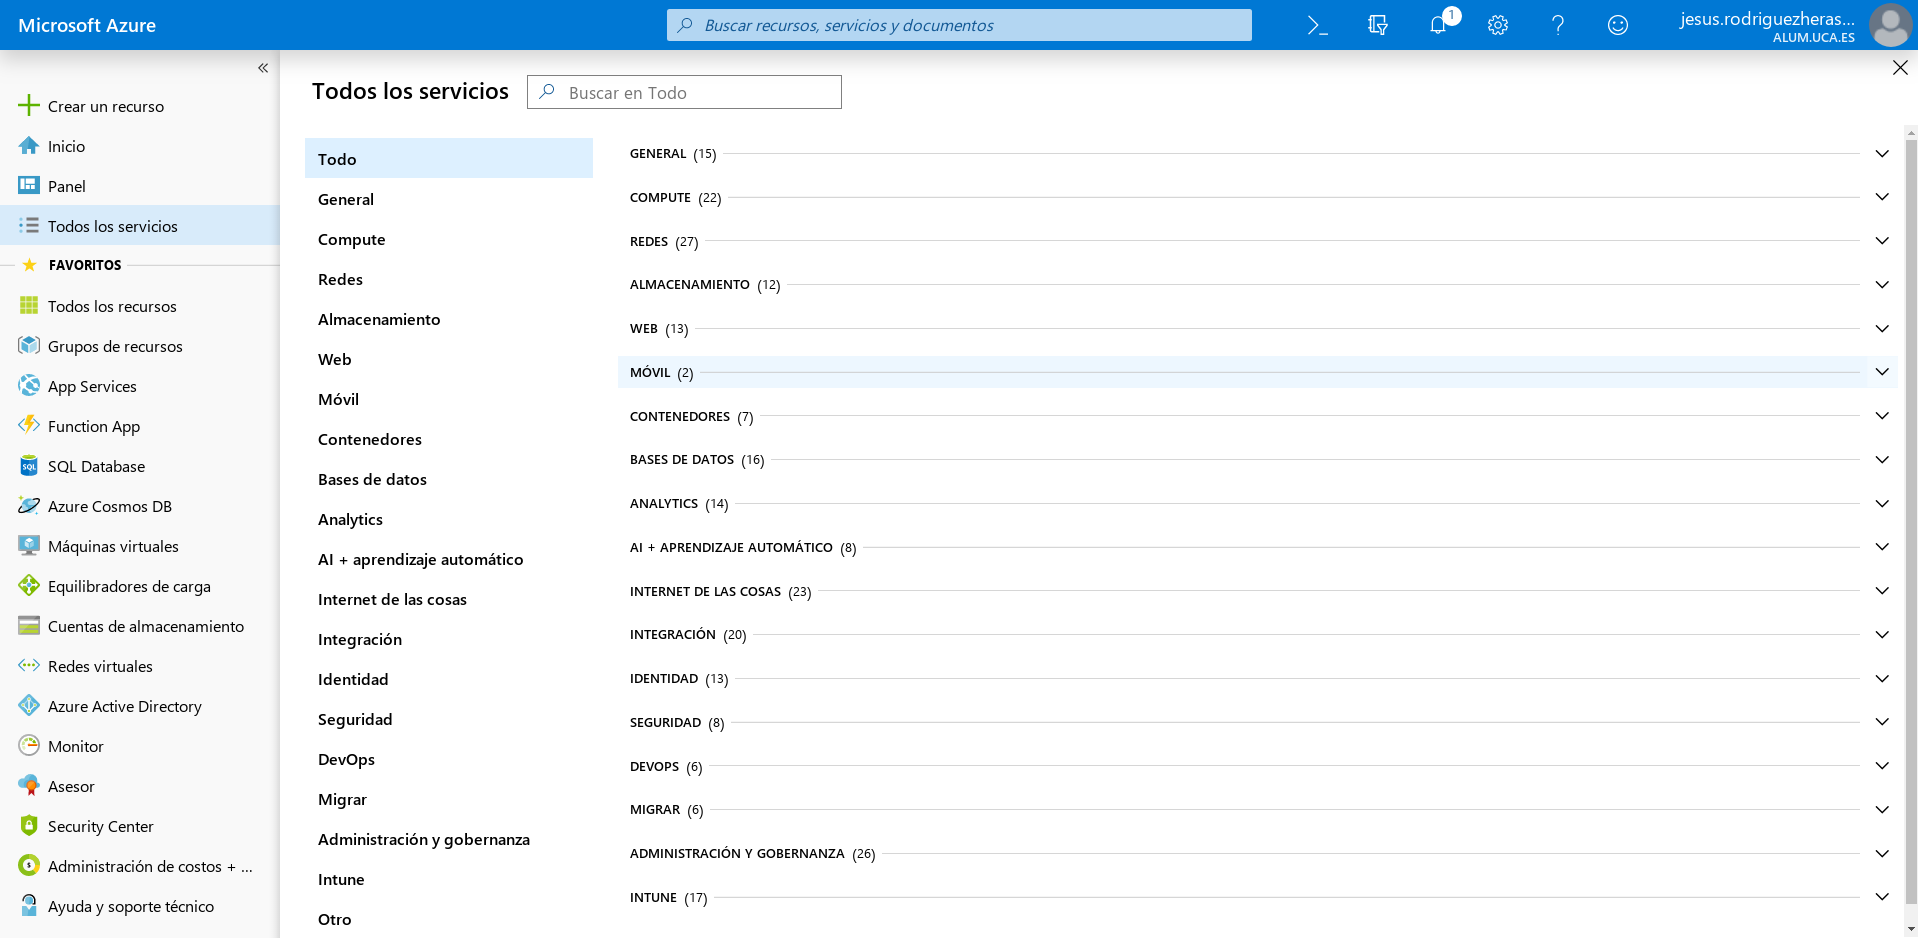
\includegraphics[scale=0.26]{ImagenesAzure/Servicios.png}
	\caption{Servicios ofrecidos por Azure.}
	\label{Servicios ofrecidos por Azure}
\end{figure}

Las características generales de Azure son las siguientes:
\begin{itemize}
	\item \textbf{Autoservicio bajo demanda:} Los usuarios pueden proveerse de cómputo en la nube sin requerir interacción humana o con el mismo proveedor.
	\item \textbf{Acceso ubicuo a la red:} Todo lo qeu podamos necesitar se encuentra en la red y accesible desde la red. Disponible desde cualquier dispositivo por medio de estándares como HTML o el protocolo HTTP.
	\item \textbf{Agrupación de recursos independientemente de la posición geográfica:} Los recursos del proveedor se encuentran geográficamente agrupados para servir a múltiples consumidores de manera distribuida y bajo demanda.
	\item \textbf{Elasticidad rápida:} Las funcionalidades se proporcionan de manera muy rápida, incluso puede ser configurable para que crezca dependiendo del ambiente actual.
	\item \textbf{Servicio medido:} El uso de todos los recursos se puede monitorizar, lo que proporciona transparencia tanto al que expone los servicios (el proveedor) como a los que acceden a ellos (los consumidores).
	\item \textbf{Pago por uso:} El costo de los servicios expuestos se puede modelar con la siguiente expresión:
	\begin{center}
		$(CaracterísticasDelServicio) * (TiempoDeActividad) = CostoTotal$
	\end{center}
\end{itemize}

Cabe destacar, y, como se ve en la figura \ref{Servicios ofrecidos por Azure} que en Azure sí contamos con servicios relacionados con Inteligencia Artificial y aprendizaje automático (Machine Learning).

\section{Limitaciones}
Dentro de la capa de estudiantes\footnote{La que hemos podido probar gracias al acuerdo de la UCA con Microsoft.} tenemos las siguientes \href{https://azure.microsoft.com/es-es/free/free-account-students-faq/}{limitaciones}, de las cuales, las más destacables son (entre muchas otras):
\begin{itemize}
	\item 750 horas de máquinas virtuales B1S\footnote{Características de las máquinas B1S: 1vCPU, 1GiB de RAM y 4GiB de almacenamiento.} tanto para Linux como para Windows.
	\item 128GB de Managed Disks\footnote{Ofrece la seguridad, disponibilidad, escalabilidad y durabilidad de HDD/SSD que se necesite para todas las cargas de trabajo, desde cargas de trabajo críticas hasta escenarios de prueba.} como combinación de dos discos de almacenamiento SSD de 64GB, además de 1GB en operaciones instantáneas y 2 millones de operaciones de E/S.
	\item 250GB de una instancia S0\footnote{Instancia de bases de datos gestionada por Azure SQL.} estándar de bases de datos SQL con 10 unidades de transacción de bases de datos.
	\item 1500 horas de IP dinámica para máquinas virtuales B1S.
\end{itemize}
	
	\part{Anexo}
	\chapter{Referencias}
En este capítulo se detallarán las referencias consultadas a la hora de redactar este documento.
\begin{itemize}
	\item Documentación oficial de AWS: \url{https://aws.amazon.com/es/}.
	\item Documentación oficial de Azure: \url{https://azure.microsoft.com/es-es/}.
	\item \url{https://es.wikipedia.org/wiki/Amazon_Web_Services}.
	\item \url{https://es.wikipedia.org/wiki/Middleware}.
	\item \url{https://revistadigital.inesem.es/informatica-y-tics/cloud-computing-con-amazon/}.
	\item \url{https://docs.aws.amazon.com/es_es/general/latest/gr/aws_service_limits.html}.
	\item \url{https://azure.microsoft.com/es-es/free/free-account-students-faq/}.
\end{itemize}
	
\end{document}
